\documentclass[11pt]{article}
%Gummi|063|=)
\title{\textbf{Algorithms I -- supervision 5}}
\author{James Wood}
\usepackage{listings}
\usepackage{bold-extra}
\usepackage{xcolor}
\usepackage{amsmath}
\usepackage{enumitem}
\usepackage{tikz}
\usetikzlibrary{arrows}

\lstset{
  basicstyle=\small,
  basewidth=0.5em,
  frame=single,
  breaklines=true,
  %postbreak=\raisebox{0ex}[0ex][0ex]{
  %  \ensuremath{\color{red}\hookrightarrow\space}
  %}
  language=python,
  literate=
    {<=}{{\(\leq\)}}1
    {>=}{{\(\geq\)}}1
    {&&}{{\(\wedge\)}}1
    {||}{{\(\vee\)}}1
    {->}{{\(\rightarrow\)}}1
}

\tikzset{
  treenode/.style = {align=center, inner sep=0pt, text centered,
    font=\sffamily},
  bnode/.style = {treenode, circle, white, draw=black,
    fill=black, text width=1.5em},
  rnode/.style = {treenode, circle, red, draw=red,
    text width=1.5em, very thick},
  leaf/.style = {treenode, rectangle, draw=black,
    minimum width=0.5em, minimum height=0.5em}
}

\begin{document}
\renewcommand{\labelenumi}{(\alph{enumi})}
\renewcommand{\labelenumii}{(\roman{enumii})}

\maketitle

\section{Hash tables}
\begin{enumerate}
\item
  \begin{tabular}[t]{r || l | l | l}
    hash & \multicolumn{3}{|c}{values} \\
    \hline
    0 & 35 & 10 & 5 \\
    1 &  6 &    & \\
    2 &  2 &    & \\
    3 & 18 &  3 & 8 \\
    4 &    &    & \\
  \end{tabular}
\item
  \begin{tabular}[t]{r || l}
    hash & value \\
    \hline
    0 & 10 \\
    1 &    \\
    2 & 2  \\
    3 & 3  \\
    4 &    \\
    5 & 35 \\
    6 & 6  \\
    7 & 5  \\
    8 & 18 \\
    9 & 8  \\
  \end{tabular}
\item
  \begin{enumerate}
  \item
    Every item in the hash table is of the form either \texttt{(key, value, next)} or \texttt{(prev, next)}, where \texttt{prev} and \texttt{next} are indices into the table. This can be represented by the algebraic data type \texttt{Entry k v i}, where \texttt k is the type of keys, \texttt v is the type of the values and \texttt i is the type of the hash function's output:
    \begin{lstlisting}[language=haskell]
data Entry k v i = Item k v (Maybe i)
                 | Free (Maybe i) (Maybe i)
    \end{lstlisting}
    Then, given \texttt{table}, an array of this type; and \texttt{firstFree}, the index in \texttt{table} of the first element in the free list, \texttt{set} is implemented as follows:
    \begin{lstlisting}
def set(key, value):
    h = hash(key)
    case table[h]:
        Item k v i:
            if k == key:
                # Replace the existing value
                table[h] = Item k value i
            else:
                # Put the new item in the place of the old one,
                # and put the old item in the first free slot
                table[h] = Item key value (Just firstFree)

                # Assuming we have more free spaces
                Free _ (Just n) = table[firstFree]
                table[firstFree] = Item k v i
                firstFree = n
        Free p n:
            # First entry for this hash value
            table[h] = Entry key value Nothing

            # Clean up free list
            case p:
                Just pi:
                    table[pi].next = n
                    case n:
                        Just ni:
                            table[ni].prev = p
                        Nothing:
                            # Do nothing
                Nothing:
                    # h == firstFree
                    # Assuming we have more free space
                    Just ni = n
                    firstFree = ni

                    table[ni].prev = Nothing
    \end{lstlisting}
  \item
    \begin{tabular}[t]{r || l | l | l | l | l | l | l | l}
      hash & 0 & 1 & 2 & 3 & 4 & \texttt{prev} & \texttt{next} & \texttt{firstFree} \\
      \hline
      0 & &      & 2, C &  2, C &  2, C &   & 1 &                \\
      1 & &      &      & 12, T & 12, T &   &   &                \\
      2 & & 2, A & 2, A &  2, A &  2, A &   & 0 &                \\
      3 & &      &      &       &       &   &   & \(\leftarrow\) \\
      4 & &      &      &       &  5, Z &   &   &                \\
    \end{tabular}
  \end{enumerate}
\end{enumerate}

\section{Red-black trees}
\begin{enumerate}
\item
  \begin{itemize}
  \item Each node is either red or black.
  \item The root is black.
  \item All (empty) leaves are black.
  \item The child of any red node is black.
  \item There exists a number \(b\) such that any path from the root to a leaf contains exactly \(b\) black nodes.
  \end{itemize}
  The main advantage of a red-black tree over a binary search tree is that no path from root to leaf can be more than twice as long as any other path from root to leaf. This means that red-black trees can't become too unbalanced, so searching is guaranteed to run in logarithmic, rather than linear, time. The main disadvantages are that red-black trees are more complex to implement and have more overhead not measured by asymptotic complexity.
\item
  2-node \([a]\):

  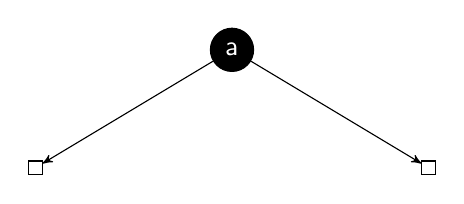
\begin{tikzpicture}[->,>=stealth',level/.style={sibling distance = 5cm/#1,level distance = 1.5cm}]
    \node[bnode]{a}
    child{node[leaf]{}}
    child{node[leaf]{}}
    ;
  \end{tikzpicture}

  3-node \([a,b]\)

  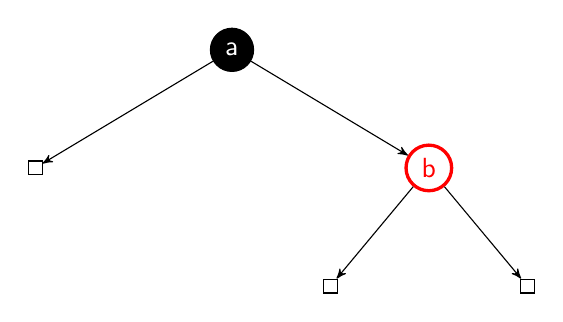
\begin{tikzpicture}[->,>=stealth',level/.style={sibling distance = 5cm/#1,level distance = 1.5cm}]
    \node[bnode]{a}
    child{node[leaf]{}}
    child{
      node[rnode]{b}
      child{node[leaf]{}}
      child{node[leaf]{}}
    }
    ;
  \end{tikzpicture}

  4-node \([a,b,c]\)

  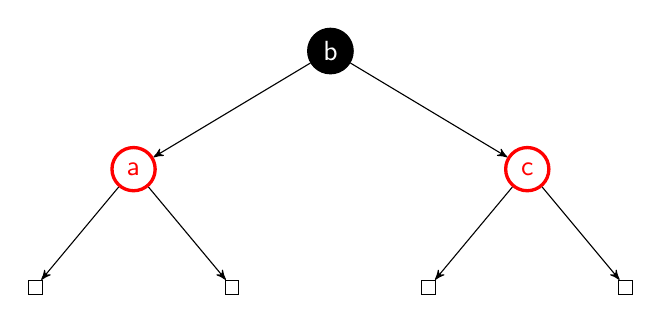
\begin{tikzpicture}[->,>=stealth',level/.style={sibling distance = 5cm/#1,level distance = 1.5cm}]
    \node[bnode]{b}
    child{
      node[rnode]{a}
      child{node[leaf]{}}
      child{node[leaf]{}}
    }
    child{
      node[rnode]{c}
      child{node[leaf]{}}
      child{node[leaf]{}}
    }
    ;
  \end{tikzpicture}
\item
  The minimum number of nodes for a given black height is achieved when there are no red nodes (since these contribute nothing to black height). This leaves a perfect binary tree of height \(h\), which has \(2^{h+1}-1\) (black) nodes.

  The maximum number of nodes for a given black height is achieved when there are as many red nodes as possible. This occurs when every other layer (starting from the layer below the root) is full of red nodes, creating a perfect tree of \(2\cdot h+1\) layers, which has \(2^{2\cdot h+2}-1\) nodes.
\item
  A rotation about a node of a binary search tree is an operation that moves one of the children of the node into its parent's place, moving the parent into the subtree opposite to the one the child came from. Then, the three subtrees of these two nodes are reättached in order. Consider this example:

  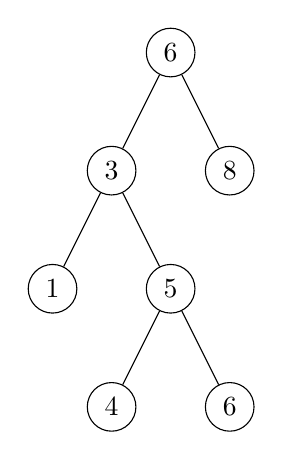
\begin{tikzpicture}
    \node[circle,draw](z){6}
    child{
      node[circle,draw]{3}
      child{node[circle,draw]{1}}
      child{
        node[circle,draw]{5}
        child{node[circle,draw]{4}}
        child{node[circle,draw]{6}}
      }
    }
    child{
      node[circle,draw]{8}
    };
  \end{tikzpicture}

  To perform a leftward rotation on the 3 node, the 5 node is moved in place of the 3 node, and the 3 node and its left subtree are reättached under the 5 node. Then, the 4 subtree is moved to become the other subtree of the 3 node, and the 6 subtree becomes the right subtree of the 5 node again. This yields:

  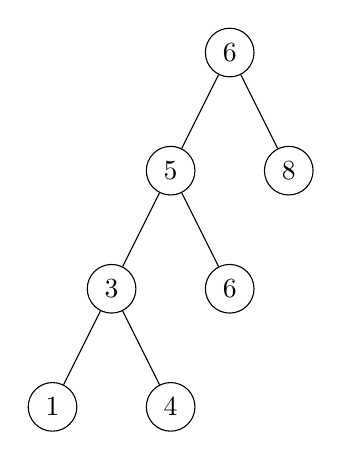
\begin{tikzpicture}
    \node[circle,draw](z){6}
    child{
      node[circle,draw]{5}
      child{
        node[circle,draw]{3}
        child{node[circle,draw]{1}}
        child{node[circle,draw]{4}}
      }
      child{node[circle,draw]{6}}
    }
    child{
      node[circle,draw]{8}
    };
  \end{tikzpicture}
\item To transform BST \(A\) into BST \(B\), find the position of \(B\)'s root's key in \(A\), then rotate this node so that it becomes the root of \(A\). At this point, the left (resp right) subtree of \(A\) will have the same keys as the left (resp right) subtree of \(B\), by the BST property. So, apply this procedure to the two subtrees recursively, with leaves (or singleton trees) already the same and acting as a base case.
\end{enumerate}

\section{Heaps}
\begin{enumerate}
\item In a min-heap, each node is less or equal to both of its children. To convert from tree to array representation, read off the elements breadth first, with some null placeholder in place of subtrees missing from the hypothetical full heap. The root has index \(0\), and a node with index \(i\) has children at \(2\cdot i+1\) and \(2\cdot i+2\).
\item When an array is sorted into ascending order, every element is less than or equal to every following element. When the array is interpreted as a tree, any element's children always follow it, and thus in a sorted array, any element's children are less or equal to it. So the heap property is satisfied.
\item
  \texttt N and \texttt L are children of \texttt R, but are smaller, so the array does not represent a min-heap. It is turned into a min-heap as follows:

  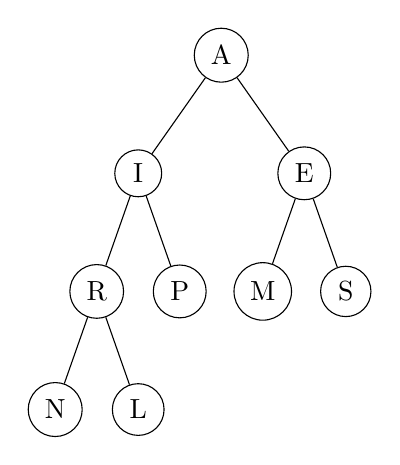
\begin{tikzpicture}[every node/.style={circle,draw},level 1/.style={sibling distance=60pt},level 2/.style={sibling distance=30pt}]
    \node(z){A}
    child{
      node{I}
      child{
        node{R}
        child{node{N}}
        child{node{L}}
      }
      child{node{P}}
    }
    child{
      node{E}
      child{node{M}}
      child{node{S}}
    };
  \end{tikzpicture}

  Start with the last element with children. If it is larger than any of its children, swap it with its smallest child, then repeat the comparison and possible swap in its new location.

  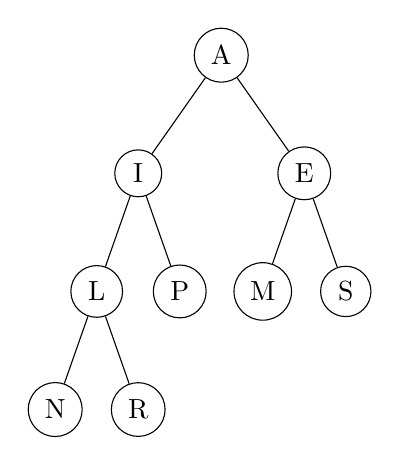
\begin{tikzpicture}[every node/.style={circle,draw},level 1/.style={sibling distance=60pt},level 2/.style={sibling distance=30pt}]
    \node(z){A}
    child{
      node{I}
      child{
        node{L}
        child{node{N}}
        child{node{R}}
      }
      child{node{P}}
    }
    child{
      node{E}
      child{node{M}}
      child{node{S}}
    };
  \end{tikzpicture}

  Then, move onto the previous element. In this case, all previous elements are in a suitable place, so there are no more intermediate steps to show.
\item
  First, the root node is removed and replaced by the last node.

  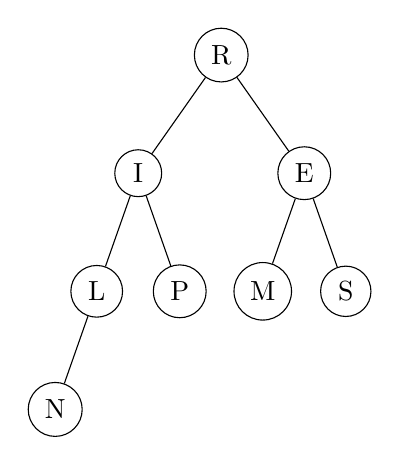
\begin{tikzpicture}[every node/.style={circle,draw},level 1/.style={sibling distance=60pt},level 2/.style={sibling distance=30pt}]
    \node(z){R}
    child{
      node{I}
      child{
        node{L}
        child{node{N}}
        child[missing]{}
      }
      child{node{P}}
    }
    child{
      node{E}
      child{node{M}}
      child{node{S}}
    };
  \end{tikzpicture}

  Then, the node that is currently the root is swapped with its smallest child until it is smaller than both of its children.

  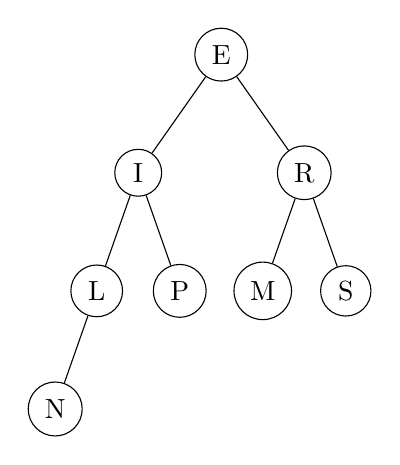
\begin{tikzpicture}[every node/.style={circle,draw},level 1/.style={sibling distance=60pt},level 2/.style={sibling distance=30pt}]
    \node(z){E}
    child{
      node{I}
      child{
        node{L}
        child{node{N}}
        child[missing]{}
      }
      child{node{P}}
    }
    child{
      node{R}
      child{node{M}}
      child{node{S}}
    };
  \end{tikzpicture}

  \texttt R needs to be moved again.

  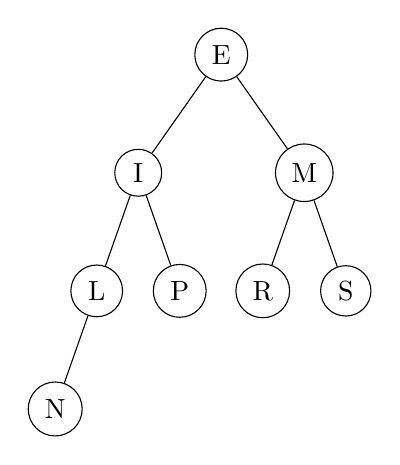
\begin{tikzpicture}[every node/.style={circle,draw},level 1/.style={sibling distance=60pt},level 2/.style={sibling distance=30pt}]
    \node(z){E}
    child{
      node{I}
      child{
        node{L}
        child{node{N}}
        child[missing]{}
      }
      child{node{P}}
    }
    child{
      node{M}
      child{node{R}}
      child{node{S}}
    };
  \end{tikzpicture}

  The min-heap property is restored.
\item Heapsort needs linear time to check that the array it is given forms a min-heap. Then, the element promoted to the top on the \texttt{extractMin} steps will always be the largest element, and thus will always need to go to the bottom of the heap, taking logarithmic time on each call. Hence, the algorithm will run in \(\Theta\,\left( n\cdot\log n \right)\) time.
\item \texttt{heapify} is known to to run in linear time. Then, when an element is promoted as part of \texttt{extractMin}, it will most likely need to be moved near the bottom of the heap, costing \(O\,\left( \log n \right)\) each time. Doing this \(n\) times gives a time complexity of \(O\,\left( n\cdot\log n \right)\).
\end{enumerate}

\section{Sorting and searching}
\begin{enumerate}
\item
  \begin{enumerate}
  \item
    Put all of the items into a priority queue, where the priority of each element is its value. Then, dequeue \(k\) elements.

    Using the heap implementation of the priority queue, building the priority queue takes \(O\,n\) time. Then, dequeueing takes \(O\,\left( k\cdot\log n \right)\) time, since it involves m oving \(k\) elements down the height of the tree. This gives worst case complexity \(O\,\left( n+k\cdot\log n \right)\).
  \item
    Assume that \(n\geq k\). If \(n=k\), return the given array. Otherwise, compare all of the elements of the array to a pivot element, putting lesser elements to the left, the pivot and equal elements after them and greater elements after those. Let \(l\) be the number of lesser elements, \(e\) be the number of elements that are or are equal to the pivot and \(g\) be the number of greater elements, so that \(l+e+g=n\). If \(k\in[0..l]\), repeat the process on the lesser elements. If \(k\in(l..l+e]\), return the first \(k\) elements currently in the array. Otherwise, in which case \(k\in(l+e..n]\), return the lesser and equal elements along with the smallest \(k-l-e\) larger elements.

    The worst cases occur when the pivot at each step is an extreme value. Then, the complexity is \(O\,\left( \max(k,n-k) \right)\). However, as with calculating order statistics, the pivot is usually not extreme, giving us the better average case of \(\Theta\,\left( \log n \right)\).
  \end{enumerate}
\item
  Sum the length fields, then pick a random number in the range \([0..s)\), where \(s\) is the sum (using \texttt{random} appropriately). Then, set \(t\) to \(s\) and iterate through the slots of the hash table, taking the length of the slot off \(t\) each time. When the length exceeds \(t\), pick the \(t\)th item in the chain of the current slot. This takes \(O\,\left( m+L \right)\) time, since it relies on traversing the slots of the hash table, then traversing a chain.
\end{enumerate}

\section{Bogosort}
\begin{enumerate}
\item
  In the best case, the list is already sorted, so the loop terminates as soon as \texttt{is\_sorted} returns. This takes \(\Theta\,n\) time.

  Any shuffling of the list has a probability of order \(1/n!\) of being sorted. Each call to \texttt{shuffle} and \texttt{is\_sorted} takes linear time. Hence, on average, bogosort will take \(\Theta\,\left(n!\cdot n\right)\), or simply \(\Theta\,\left(n!\right)\), time.

  Bogosort is not guaranteed to terminate, so has undefined worst case complexity.
\item Bogosort is unstable because there are no guarantees based on the order of the input list on the order of the output list.
\end{enumerate}

\end{document}